\documentclass[aspectratio=169]{beamer}
\usepackage[no-math,deluxe,haranoaji]{luatexja-preset}
\renewcommand{\kanjifamilydefault}{\gtdefault}
\renewcommand{\emph}[1]{{\upshape\bfseries #1}}
\usetheme{metropolis}
\metroset{block=fill}
\setbeamertemplate{navigation symbols}{}
\usecolortheme[rgb={0.7,0.2,0.2}]{structure}
%%%%%%%%%%%%%%%%%%%%%%%%%%%
\usepackage{media9}
%%%%%%%%%%%%%%%%%%%%%%%%%%%
%% さまざまなアイコン
%%%%%%%%%%%%%%%%%%%%%%%%%%%
\usepackage{fontawesome}
\usepackage{figchild}
\usepackage{twemojis}
\usepackage{utfsym}
\usepackage{bclogo}
\usepackage{marvosym}
%%%%%%%%%%%%%%%%%%%%%%%%%%%
\usepackage{tikz}
\usetikzlibrary{backgrounds}
\usepackage{tcolorbox}
\usepackage{tikzpeople}
\usepackage{xcolor}
\usepackage{amsmath}
%%%%%%%%%%%%%%%%%%%%%%%%%%%
%% 場合分け
\usepackage{cases}
%%%%%%%%%%%%%%%%%%%%%%%%%%%
% \myAnch{<名前>}{<色>}{<テキスト>}
% 指定のテキストを指定の色の四角枠で囲み, 指定の名前をもつTikZの
% ノードとして出力する. 図には remeber picture 属性を付けている
% ので外部から参照可能である.
\newcommand*{\myAnch}[3]{%
  \tikz[remember picture,baseline=(#1.base)]
    \node[draw,rectangle,#2] (#1) {\normalcolor #3};
}
%%%%%%%%%%%%%%%%%%%%%%%%%%%%
%% 音声リンク表示
\newcommand{\myaudio}[1]{\href{#1}{\faVolumeUp}}
%%%%%%%%%%%%%%%%%%%%%%%%%%%
% \myEmph コマンドの定義
%\newcommand{\myEmph}[3]{%
%    \textbf<#1>{\color<#1>{#2}{#3}}%
%}
\usepackage{xparse} % xparseパッケージの読み込み
\NewDocumentCommand{\myEmph}{O{} m m}{%
    \def\argOne{#1}%
    \ifx\argOne\empty
        \textbf{\color{#2}{#3}}% オプション引数が省略された場合
    \else
        \textbf<#1>{\color<#1>{#2}{#3}}% オプション引数が指定された場合
    \fi
}
%%%%%%%%%%%%%%%%%%%%%%%%%%%
\title{English is fun.\,\,{}---A Tale of Two cities---}
\author{}
\institute[]{}
\date[]

%%%%%%%%%%%%%%%%%%%%%%%%%%%%
%% TEXT
%%%%%%%%%%%%%%%%%%%%%%%%%%%%
\begin{document}
\begin{frame}[plain]
  \titlepage
\end{frame}

\section*{授業の流れ}
\begin{frame}[plain]
  \frametitle{授業の流れ}
  \tableofcontents
\end{frame}

\section{単数と複数}

\begin{frame}[plain]\frametitle{ひとつとふたつ以上}
\begin{columns}
\begin{column}{.25\textwidth}
\IfFileExists{./images/one_book-crop.pdf}{%
\rotatebox{-90}{\includegraphics[width=1.1\textwidth]{./images/one_book-crop.pdf}
}}{naiyo}
\end{column}\pause
\begin{column}{.5\textwidth}\LARGE
a book
\end{column}
\end{columns}

\pause
\begin{columns}
\begin{column}{.25\textwidth}
\IfFileExists{./images/two_books-crop.pdf}{%
\rotatebox{-90}{\includegraphics[width=1.1\textwidth]{./images/two_books-crop.pdf}
}}{naiyo}
\end{column}\pause
\begin{column}{.5\textwidth}\LARGE
two book\myEmph[4]{orange}{s}
\end{column}

\end{columns}
\end{frame}



\subsection{日本語とのちがい}
\begin{frame}<1-10>[plain]\frametitle{日本語とのちがい}
\begin{columns}
\begin{column}[t]{.45\textwidth}
\begin{block}{日本語}
\onslide<2->{わたしは1冊の本を持っています。}

\onslide<3->{わたしは2冊の本を持っています。}

\onslide<4->{わたしは本を持っています。}
\end{block}
\end{column}
\begin{column}[t]{.45\textwidth}
\begin{block}{英語}
\onslide<5->{I have \textcolor{orange}{a book.}}

\onslide<6->{I have \textcolor{orange}{two books.}}

\onslide<7->*{I have \textcolor{red!50}{book}.}\onslide<8>{\,\,{}$\longleftarrow$これは\textcolor{red}{だめ}}
\end{block}
\end{column}
\end{columns}

\begin{exampleblock}<9->{Topics for Today}
\begin{itemize}
 \item<1->  \onslide<9,10>{\textcolor{orange}{単数形と複数形があります}}
 \item<2->  \onslide<10>{\textcolor{orange}{単数形を裸で使うことはできません}}
\end{itemize}
      \end{exampleblock}

\end{frame}

\section{複数形のつくり方}
\subsection{基本}
\begin{frame}[plain]\frametitle{複数形のつくり方}
 
\Large
おしりに---sをつけます。

a book $\longrightarrow$ book\textcolor{orange}{s}

\end{frame}



\subsection{Exercises}
\begin{frame}[plain]\frametitle{Exercises}

\fcDog{0.4}{black}{1}\pause a dog\hspace{20pt}%
\pause
\fcDog{0.4}{black}{1}\fcDog{0.4}{black}{1}\pause two dogs
\pause

\fcCat{0.4}{black}{1}\pause a cat\hspace{40pt}%
\pause
\fcCat{0.4}{black}{1}\fcCat{0.4}{black}{1}\fcCat{0.4}{black}{1} \pause three cats
\pause

\fcBirdB{0.4}{black}{1}\pause a bird\hspace{45pt}%
\pause
\fcBirdB{0.4}{black}{1}
\fcBirdB{0.4}{black}{1}
\fcBirdB{0.4}{black}{1}
\fcBirdB{0.4}{black}{1} \pause four birds

\end{frame}


\begin{frame}[plain]\frametitle{Exercises(Continued)}

\fcBookB{0.4}{black}{1}\pause a book\hspace{20pt}%
\pause
\fcBookB{0.4}{black}{1}\fcBookB{0.4}{black}{1}%
\fcBookB{0.4}{black}{1}\fcBookB{0.4}{black}{1}%
\fcBookB{0.4}{black}{1} \pause five books
\pause

\bigskip

\scalebox{.17}{\fcKey{0.4}{black}{2}}\,\,{}\pause a key\hspace{40pt}%
\pause
\scalebox{.17}{\fcKey{0.4}{black}{2}} \scalebox{.17}{\fcKey{0.4}{black}{2}} \scalebox{.17}{\fcKey{0.4}{black}{2}} \scalebox{.17}{\fcKey{0.4}{black}{2}} \scalebox{.17}{\fcKey{0.4}{black}{2}} \scalebox{.17}{\fcKey{0.4}{black}{2}}
\pause
 six keys
\pause

\scalebox{.25}{\fcChairA{0.4}{black}{2}}\pause a chair\hspace{40pt}%
\pause
\scalebox{.25}{\fcChairA{0.4}{black}{2} \fcChairA{0.4}{black}{2} \fcChairA{0.4}{black}{2} \fcChairA{0.4}{black}{2} \fcChairA{0.4}{black}{2} \fcChairA{0.4}{black}{2} \fcChairA{0.4}{black}{2}}
\pause
 seven chairs
\pause

\scalebox{1}{\fcBike{0.4}{black}{1}}\pause a bike\hspace{30pt}%
\pause
\scalebox{1}{\begin{tabular}{@{}lllll}
\fcBike{0.4}{black}{1}& \fcBike{0.4}{black}{1}& \fcBike{0.4}{black}{1}& \fcBike{0.4}{black}{1}& \fcBike{0.4}{black}{1}\\
 \fcBike{0.4}{black}{1}& \fcBike{0.4}{black}{1}& \fcBike{0.4}{black}{1}
	     \end{tabular}}
\pause
\mbox{}\hspace*{.8\textwidth} eight bikes
\end{frame}


\begin{frame}[plain]\frametitle{Exercises(Continued)}

\usymW{2710}{1cm}\pause a pencil\hspace{20pt}%
\pause
\usymW{2710}{1cm}\usymW{2710}{1cm}\usymW{2710}{1cm}\usymW{2710}{1cm}\usymW{2710}{1cm}\hspace{15pt}
\usymW{2710}{1cm}\usymW{2710}{1cm}\usymW{2710}{1cm}\usymW{2710}{1cm}\pause

\mbox{}\hspace{.8\textwidth} nine pencils
\pause


\bcfleur\,\,\,\,\pause a flower\hspace{45pt}%
\pause
\bcfleur\bcfleur\bcfleur\bcfleur\bcfleur\hspace{15pt}
\bcfleur\bcfleur\bcfleur\bcfleur\bcfleur\hspace{10pt}
\pause
ten flowers
\end{frame}


\begin{frame}[plain]\frametitle{Pronunciation}

\begin{enumerate}
 \item a dog~~~/~~~two dogs
 \item a cat~~~/~~~three cats
 \item a bird~~~~/~~~four birds
 \item a book~~~/~~~five books
 \item a key~~~/~~~six keys
 \item a chair~~~/~~~seven chairs
 \item a bike~~~/~~~eight bikes
 \item a pencil~~~~/~~~nine pencils
 \item a flower~~~/~~~ten flowers
\end{enumerate}

% Embed the sound file
\pause
\myaudio{./audio/005_singular_plural_01.mp3}\,\,{}Listen carefully.(注意して聞いてください)

\end{frame}

\subsection{注意すべき複数形}

\begin{frame}[plain]{注意すべき複数形}

\scalebox{.5}{\fcBus{0.4}{black}{2}}\hspace{15pt}\pause {\LARGE a bus}
\pause

\bigskip

\bigskip

\scalebox{.5}{\fcBus{0.4}{black}{2}\hspace{15pt}\fcBus{0.4}{black}{2}}\hspace{15pt}
\pause {\LARGE two  bus\textcolor{orange}{es}}
\end{frame}

\begin{frame}[plain]{注意すべき複数形}
\scalebox{.4}{\fcPotato{0.4}{black}{2}}\hspace{15pt}
\pause
{\LARGE a potato}
\pause

\bigskip

\bigskip

\scalebox{.4}{\fcPotato{0.4}{black}{2}\hspace{15pt}\fcPotato{0.4}{black}{2}}\hspace{15pt}
\pause
{\LARGE two  potato\textcolor{orange}{es}}
\end{frame}

\begin{frame}[plain]\frametitle{注意すべき複数形}

{\Large `s'ではなく\textcolor{orange}{`es'}をつける複数形があります}
\pause

\bigskip

\begin{block}{--- $\rightarrow$ ---es}

a bus \pause$\longrightarrow$ bus\textcolor{orange}{es}\pause

a potato \pause$\longrightarrow$ potato\textcolor{orange}{es}\pause

a tomato \pause$\longrightarrow$ tomato\textcolor{orange}{es}\pause

a class \pause$\longrightarrow$ class\textcolor{orange}{es}\pause

a box\pause $\longrightarrow$ box\textcolor{orange}{es}
\end{block}

\end{frame}


\begin{frame}[plain]\frametitle{Pronunciation}

\begin{enumerate}
 \item a bus~~~\pause{}/~~~buses\pause
 \item a potato~~~\pause{}/~~~potatoes\pause
 \item a tomato~~~\pause{}/~~~tomatoes\pause
 \item a class~~~~\pause{}/~~~classes\pause
 \item a box~~~\pause{}/~~~boxes
 \end{enumerate}
\pause
\myaudio{./audio/005_singular_plural_02.mp3}\,\,{}Listen carefully.(注意して聞いてください)
\end{frame}


\begin{frame}[plain]{注意すべき複数形}
\scalebox{5}{\ManFace}\hspace{15pt}
\pause
{\LARGE a man}
\pause

\bigskip

\bigskip

\scalebox{5}{\ManFace\hspace{5pt}\ManFace\hspace{5pt}\ManFace}\hspace{15pt}
\pause
{\LARGE three  \textcolor{orange}{men}}
\end{frame}

\begin{frame}[plain]{注意すべき複数形}
\scalebox{5}{\WomanFace}\pause\hspace{15pt} {\LARGE a woman}
\pause

\bigskip

\bigskip

\scalebox{5}{\WomanFace \WomanFace \WomanFace \WomanFace} \hspace{25pt}
\pause
{\LARGE four  \textcolor{orange}{women}}
\end{frame}

\begin{frame}[plain]{注意すべき複数形}
\scalebox{.7}{%
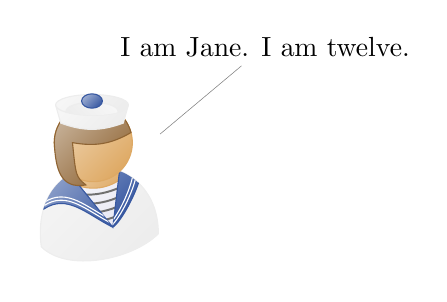
\begin{tikzpicture}
\node[sailor,female,minimum size=1.5cm,
anchor=south,pin={85:I am Jane. I am twelve.}] at (6.25cm,0) {};
%\node[charlie,minimum size=1.5cm,
%anchor=south,,pin={105:I am Bob.}] at (5cm,0) {};
\end{tikzpicture}
}\pause
\hspace{80pt}{\Large a child}
\pause

\bigskip

\scalebox{.7}{%
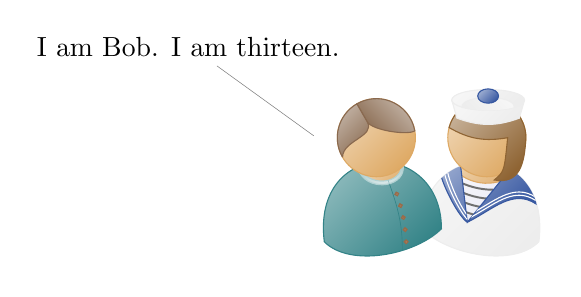
\begin{tikzpicture}
\node[sailor,female,mirrored,minimum size=1.5cm,
anchor=south] at (6.25cm,0) {};
\node[charlie,minimum size=1.5cm,
anchor=south,,pin={105:I am Bob. I am thirteen.}] at (5cm,0) {};
\end{tikzpicture}
}\pause
\hspace{45pt}{\Large two \textcolor{orange}{children}}

\end{frame}


\begin{frame}[plain]\frametitle{Pronunciation}

\begin{enumerate}
 \item a man~~~\pause{}/~~~men\pause
 \item a woman~~~\pause{}/~~~women\pause
 \item a child~~~\pause{}/~~~children
  \end{enumerate}
\pause
\myaudio{./audio/005_singular_plural_03.mp3}\,\,{}Listen carefully.(注意して聞いてください)
\end{frame}



\begin{frame}<1-9>[plain]\frametitle{Exercises}
空所に適当な動詞を補ってください。なお、必要があれば、形を変えてください

 % \setbeamercovered{transparent}
  \begin{enumerate}
   \item George (\onslide<2,8,9>{\textcolor{orange}{~has~}}) two cats.
{\footnotesize ジョージはネコを2匹飼っています。}
   \item My mother (\onslide<3,8,9>{\textcolor{orange}{~teaches~}}) music.{\footnotesize 母は音楽を教えています。}
   \item  She (\onslide<4,8,9>{\textcolor{orange}{~washes~}}) her car every Saturday.{\footnotesize 彼女は毎週土曜日に洗車します。}
   \item Tom (\onslide<5,8,9>{\textcolor{orange}{~goes~}}) to church every Sunday.{\footnotesize トムは毎週日曜日に教会へ行きます。}
   \item Jennifer (\onslide<6,8,9>{\textcolor{orange}{~watches~}}) television after supper.{\footnotesize ジェニファーは夕食後テレビをみます。}
   \item He (\onslide<7,8,9>{\textcolor{orange}{~studies~}}) English every day.{\footnotesize 彼は毎日英語を勉強します。} \onslide<9>{\textcolor{orange}{studyの3単現はstdies}}
  \end{enumerate}

\begin{tcolorbox}[title=この中から選んでください]
\centering
 watch,~~~~~~~~study,~~~~~~~~have,~~~~~~~~teach,~~~~~~~~go,~~~~~~~~wash
\end{tcolorbox}

% Embed the sound file
\onslide<9>{%
\myaudio{audio/004_verb_05.mp3}\,\,{}Listen carefully.(注意して聞いてください)

}
\end{frame}

\begin{frame}<1-37>[plain,label=example]\frametitle{単数と複数}
 % \setbeamercovered{transparent}
  \begin{enumerate}
   \item<1-> \myEmph[14]{red}{I} \myEmph[15,27-29]{blue}{like} basketball. \onslide*<2>{わたしはバスケットボールが好きです。}\onslide*<31>{\footnotesize  like: 好き、好む basketball: バスケットボール}
   \item<3-> \myEmph[16]{red}{We} \myEmph[17,27-29]{blue}{walk} to school. \onslide*<4>{われわれは歩いて学校へ行きます。}\onslide*<32>{\footnotesize  walk: 歩く}
   \item<5-> \myEmph[18]{red}{They} \myEmph[19,27-29]{blue}{speak} English in Australia. \onslide*<6>{オースタラリアでは英語が話されています。}\onslide*<33>{\footnotesize  speak: 話す Australia:オーストラリア}
   \item<7-> \myEmph[20]{red}{I} \myEmph[21,27-29]{blue}{drink} tea every morning. \onslide*<8>{わたしは毎朝お茶を飲みます。}\onslide*<34>{\footnotesize  drink: 飲む tea: お茶 every morning: 毎朝}
   \item<9-> \myEmph[22]{red}{They} \myEmph[23,27-29]{blue}{study} math every day. \onslide*<10>{彼らは毎日数学を勉強します。}\onslide*<35>{\footnotesize study: 勉強する math: 数学 every day: 毎日}
   \item<11-> \myEmph[24]{red}{I} \myEmph[25,27-29]{blue}{play} the guitar. \onslide*<12>{わたしはギターをひきます。}\onslide*<36>{\footnotesize  play: (楽器などを)演奏する guitar: ギター}
  \end{enumerate}

\bigskip

\begin{exampleblock}<28->{Topics for Today}
\begin{itemize}
 \item<1->  \myEmph[28]{orange}{be動詞以外を一般動詞といいます}
 \item<2-> \myEmph[29]{orange}{一般動詞の意味はいろいろです}
\end{itemize}
      \end{exampleblock}


% Embed the sound file
\onslide<37>{%
\myaudio{./audio/004_verb_01.mp3}\,\,{}Listen carefully.(注意して聞いてください)
}

\end{frame}

\end{document}
